\cleardoublepage
\chapter{Tecnologías, Herramientas y Metodologías}

% Descripción de los lenguajes de programación, entornos de desarrollo, herramientas auxiliares, librerías de terceros, sistemas operativos, navegadores web, etc. utilizados para la realización del proyecto, así como la metodología empleada. El grado de profundidad a la hora de explicar cada tecnología dependerá de lo relevante que ha sido para el proyecto y lo conocida que es. Por ejemplo, si se usa el lenguaje de programación Java, no es necesario entrar en tanto detalle como si se usa un lenguaje mucho menos usado como Scala, por ejemplo.

% Respecto a la metodología, dada la naturaleza de los proyectos, se suele describir una metodología iterativa e incremental en espiral, en la que se van sucediendo reuniones con el profesor que van definiendo el ámbito del proyecto.

% Este capítulo puede tener una extensión entre 10 y 15 páginas.

\section{Lenguaje de programación}

Para implementar una aplicación nativa en Android se puede usar como lenguaje de programacion Java o Kotlin.
El desarrollo de Pinche se ha realizado utilizando Kotlin \cite{kotlin}.

Las principales razones por las que se ha decidido usar Kotlin para el desarrollo de esta aplicación frente a Java son:

\begin{itemize}
    \item \textbf{Sintaxis más concisa y expresiva}: Kotlin permite reducir la cantidad de código, optimizando la implementación. Por ejemplo, la gestión de getters/setters, estructuras de datos y operaciones sobre colecciones se realiza de forma mucho más directa y legible.

    \item \textbf{Seguridad frente a errores de null}: Kotlin incluye un sistema de tipos que distingue claramente entre referencias anulables y no anulables, lo que reduce la probabilidad de errores en tiempo de ejecución relacionados con punteros nulos (el conocido \textit{NullPointerException} en Java).

    \item \textbf{Interoperabilidad con Java}: Kotlin es totalmente interoperable con Java, lo que permite utilizar bibliotecas existentes. Esto es especialmente útil en Android, ya que muchas APIs aún están escritas en Java.

    \item \textbf{Compatibilidad con herramientas modernas de Android}: Kotlin se integra de forma nativa con bibliotecas modernas como Jetpack Compose, Hilt, Coroutines o Navigation, lo que simplifica el uso de arquitecturas modernas (como MVVM) y prácticas de desarrollo actuales.

    \item \textbf{Soporte oficial, comunidad y futuro garantizado}: Google ha declarado que “Android is Kotlin-first”, lo que coloca a Kotlin como lenguaje oficial recomendado.
\end{itemize}

\section{Frameworks y librerías}

\subsection{Jetpack Compose}

Para la construcción de la interfaz de usuario se ha utilizado \textbf{Jetpack Compose}, el framework de Android más moderno para crear interfaces de forma declarativa. Su primera versión estable fue lanzada en 2020. Esta elección responde a usar herramientas actuales, recomendadas por Google, que permiten mayor productividad y fluidez en el desarrollo.

Durante mucho tiempo, el desarrollo de interfaces en Android se ha basado en el uso de archivos \texttt{XML} que describen los elementos de la interfaz de forma estática, combinados con código Java o Kotlin para enlazar y actualizar esos elementos en tiempo de ejecución. Este enfoque impone una separación forzada entre lógica e interfaz, que complica la sincronización entre los datos y la vista.

\textbf{Jetpack Compose} rompe con este modelo tradicional al introducir una forma de construir la UI de manera totalmente \textbf{declarativa}, es decir, describiendo \textit{qué} debe mostrarse en lugar de \textit{cómo} hacerlo paso a paso. La interfaz se define directamente en Kotlin, mediante funciones composables, lo que permite una mejor integración con la lógica de negocio, la reutilización de componentes y mejora la legibilidad del código \cite{jetpack}.

Entre las principales ventajas de Jetpack Compose frente a XML destacan:

\begin{itemize}
    \item \textbf{Menor complejidad}: No es necesario gestionar manualmente el enlace entre XML y el resto del código. La UI responde automáticamente a los cambios de estado.

    \item \textbf{Código más conciso y reutilizable}: Al trabajar con funciones composables de Kotlin, se pueden componer interfaces complejas a partir de pequeños componentes reutilizables.

    \item \textbf{Mejor integración con la arquitectura moderna}: Compose se integra de forma nativa con patrones como MVVM que es el que seguimos en este proyecto, flujos reactivos como StateFlow para manejar estados e incluso herramientas de testing específicas para UI.

    \item \textbf{Vista previa en tiempo real}: Android Studio permite visualizar cambios en la UI mientras se escribe el código, lo que acelera el diseño y validación de pantallas. A diferencia de XML con el que hay que construir la aplicación cada vez que quieras ver el impacto de un cambio.

    \item \textbf{Mantenimiento más sencillo}: Al eliminar el archivo XML y mantener toda la lógica en un solo lenguaje, se reduce el esfuerzo de mantenimiento y depuración.
\end{itemize}

\subsection{Jetpack Navigation}

Para la gestión de la navegación entre pantallas se ha utilizado \textbf{Jetpack Navigation}, que permite definir flujos de navegación mediante un grafo centralizado, asegurando la coherencia del estado de la aplicación y facilitando el paso de argumentos entre distintas pantallas y componentes \cite{jetpack-navigation}.

\subsection{Coroutines}

\subsection{Hilt}

Con el objetivo de aportar robustez y escalabilidad a la aplicación, \textbf{Hilt} se ha intregado como sistema de \textit{inyección de dependencias}. Esto permite simplificar la gestión de instancias y facilitar su sustitución por instancias de prueba para llevar a cabo los test. También se ha tenido en cuenta su integración con el ciclo de vida recomendado de Android y su compatibilidad con Jetpack \cite{hilt}.

\section{Firebase}

\textbf{Firebase}, de Google, es una plataforma de desarrollo de aplicaciones que proporciona una serie de servicios backend listos para usar: bases de datos en tiempo real, autenticación de usuarios, almacenamiento en la nube, análisis, herramientas de pruebas y despliegue. Está pensada especialmente para aplicaciones móviles y web. Su uso agiliza significamente el desarrollo del backend en aplicaciones \cite{firebase}.

En este proyecto se utilizan principalmente dos componentes clave de Firebase:

\begin{itemize}
    \item \textbf{Firebase Authentication:} permite implementar de forma sencilla el mecanismo de registro y acceso mediante email y contraseña que hemos utilizado en Pinche \cite{firebase-auth}.

    \item \textbf{Cloud Firestore:} una base de datos NoSQL que permite almacenar y sincronizar datos en tiempo real entre los dispositivos de los usuarios y la nube, con una estructura basada en colecciones y documentos \cite{firestore}.
\end{itemize}

Una de las principales ventajas de Firebase es su integración nativa con Android, lo que simplifica su uso desde Kotlin, además de su escalabilidad y su soporte para herramientas de desarrollo como Android Studio y \textit{Firebase Emulator Suite}, que permite hacer pruebas locales de testeo sin impactar en la base de datos real \cite{firebase-emulator}.

\section{Entorno de desarrollo}

El entorno de desarrollo utilizado ha sido \textbf{Android Studio}, IDE oficial de Android. Proporciona herramientas avanzadas como el emulador y da soporte completo para Compose, Kotlin y Firebase. Para las pruebas de la app se han utilizado tanto emuladores como un dispositivo físico \cite{android-studio}.

\section{Control de versiones}

Para la gestión del código fuente se ha utilizado el conocido sistema de control de versiones \textbf{Git} y \textbf{GitHub} como repositorio remoto. El trabajo se ha organizado siguiendo prácticas comunes en entornos colaborativos. Esto ha permitido mantener versiones estables y realizar integraciones progresivas de nuevas funcionalidades. El flujo de trabajo ha sido el siguiente: se han creado ramas para la implementación de tareas concretas, por ejemplo: \texttt{feature/login}, una vez finalizada la tarea y testeada de manera atómica su funcionalidad se mergea en la rama \texttt{dev} donde se comprueba que la nueva funcionalidad no afecta a las implementadas anteriormente y tras las comprobaciones se realiza la actualizacion de la rama \texttt{main} que es la rama estable del proyecto \cite{git} \cite{github}.

\section{Metodologías de desarrollo}

Para la definición, la planificación y el desarrollo de la Pinche utilizaremos la combinación de tres metodologías complementarias y actualmente en auge: Design Thinking, Lean Startup y Agile. El ciclo de combinar estas tres metodologías se explica visualmente en la Figura~\ref{fig:methodologies}.

\begin{figure}[H]
\centering
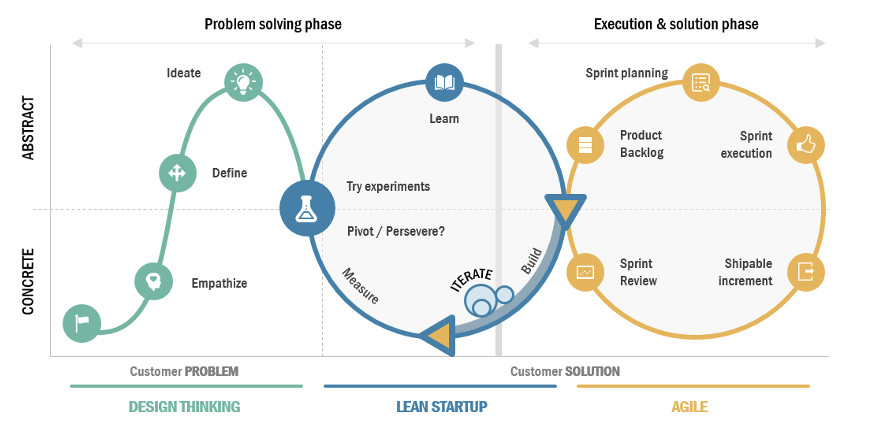
\includegraphics[width=0.9\textwidth]{./img/methodologies/methodologies.png}
\caption{Ciclo de combinar Design Thinking, Lean Startup y Agile.  Fuente: \href{https://www.gartner.com/en}{Gartner}}
\label{fig:methodologies}
\end{figure}

Por supuesto, una parte importante de esta fase será adaptar las metodologías a nuestro proyecto y a nuestro objetivo, sin perdernos en intentar aplicar cada una de manera estricta, de manera que agilicen la puesta en marcha de la solución.

\subsection{Design Thinking}

Durante la fase inicial se aplicó el enfoque de \textbf{Design Thinking}. Su objetivo es generar soluciones para un problema concreto teniendo siempre el foco en el usuario. Se siguen cinco fases: empatía, definición, prototipado y validación \cite{designthinking}. Se ha aplicado la técnica de los seis sombreros (Six Thinking Hats) que ofrece un enfoque estructurado en el que se discuten las soluciones desde seis perspectivas distintas, una por sombrero: perspectiva objetiva (sombrero blanco), perspectiva crítica y negativa (sombrero negro), perspectiva creativa (sombrero verde), perspectiva emocional (sombrero rojo), perspectiva optimista (sombrero amarillo) y perspectiva de control y gestión del proceso (sombrero azul) \cite{six-thinking-hats}.

\subsection{Lean Startup}

\textbf{Lean Startup} es una metodología que ayuda al desarrollo de productos o servicios de manera ágil, reduciendo los riesgos, promoviendo el aprendizaje y disminuyendo el tiempo de lanzamiento. Todo esto contribuye también a reducir los gastos y riesgos, al situar al cliente real en el centro de todas las decisiones de desarrollo \cite{leanstartup}.

Los principios fundamentales de Lean Startup son:

\begin{itemize}
  \item \textbf{Producto Mínimo Viable (MVP)}: Se definen unas hipótesis a confirmar y se genera una versión básica del producto que cubra la funcionalidad necesaria para comprobar dichas hipótesis y redirigir la definición del producto según lo que funciona y lo que no.

  \item \textbf{Construir, medir y aprender}: Se construye el MVP, se mide su desempeño y aceptación por parte del usuario, se recopilan datos y se decide en base a ellos. Este ciclo se repite durante toda la definición del producto.

  \item \textbf{Experimentación continua}: Se evalúa constantemente el producto o servicio, de manera que no hay un plan fijo de acción ni se comprometen recursos desde el principio.

  \item \textbf{Iteraciones rápidas}: La generación de MVPs debe ser ágil, demostrando flexibilidad a la hora de aplicar los cambios necesarios tras la última iteración.

  \item \textbf{Validación de hipótesis}: Se utilizan métricas y datos que ayudan a vislumbrar si una idea de negocio tiene mercado o no, evitando el gasto innecesario de recursos.
\end{itemize}

\subsection{Agile}

La metodología \textbf{Agile} se centra en la flexibilidad, la colaboración y la entrega incremental de valor al cliente durante el desarrollo de un proyecto. Con esta metodología se pretende generar una mayor adaptabilidad frente a los cambios que surgen durante el desarrollo, reduciendo los tiempos de entrega y mejorando la calidad del producto.

Agile se basa en el \textit{Manifiesto Ágil}, publicado en 2001, que consta de cuatro valores principales y doce principios \cite{agile-manifest} \cite{agile-manifest-principles}.

\paragraph{Valores del Manifiesto Ágil:}
\begin{itemize}
    \item Individuos e interacciones frente a procesos y herramientas.
    \item Software funcional sobre documentación extensiva.
    \item Colaboración con el cliente frente a negociación de contratos.
    \item Responder ágilmente al cambio frente a seguir un plan rígido.
\end{itemize}

\paragraph{Principios:}
\begin{itemize}
    \item Satisfacer al cliente mediante la entrega rápida y continua de software funcional.
    \item Aceptar los cambios, los requisitos por cumplir pueden ser incluidos en cualquier etapa del desarrollo.
    \item Entregar frecuentemente un producto funcional, en ciclos cortos de tiempo.
    \item Colaboración constante con el cliente para asegurar que se cubren todas sus necesidades.
    \item Motivar a los equipos de trabajo para fomentar su implicación y confianza.
    \item Comunicación cara a cara como medio más eficiente y efectivo.
    \item Valorar el software funcional como principal medida de progreso.
    \item Sostenibilidad mediante una velocidad constante y sostenible para que el ritmo al que trabaja el equipo sea accesible.
    \item Atención a la excelencia técnica y al buen diseño.
    \item Simplicidad, eliminando lo innecesario o lo que no aporta valor real.
    \item Equipos autoorganizados con capacidad de decisión.
    \item Revisión y ajuste constantes para mejorar la efectividad.
\end{itemize}

Algunas metodologías que surgen del enfoque Agile son \textbf{Scrum}, \textbf{Kanban} y \textbf{Extreme Programming (XP)}.

\paragraph{Scrum.} Es una metodología de trabajo que permite el manejo de proyectos complejos permitiendo que los equipos trabajen de manera iterativa e incremental. El trabajo se organiza en \textbf{Sprints}, que son ciclos cortos de tiempo que tienen como objetivo un incremento funcional del producto que el equipo está desarrollando \cite{scrum}.

Entre sus principales elementos dentro de la metodología Scrum encontramos roles claves como Product Owner, Scrum Master y el equipo de desarrollo. El \textbf{Product Owner} define cuáles son las prioridades que maximizan el valor del producto. El \textbf{Scrum Master} facilita el proceso Scrum y se asegura de que se aplica correctamente. Y, por último, el \textbf{equipo de desarrollo} es el encargado de implementar el producto.

Dentro de esta metodología también encontramos elementos o herramientas clave que facilitan su aplicación: \textbf{Product Backlog}, una lista priorizada de todas las tareas del proyecto, \textbf{Sprint Backlog}, que abarca todas las tareas a realizar en un sprint, y el \textbf{incremento} que sería el producto funcional que entrega el equipo de desarrollo al final de cada sprint.

Para la gestión del tiempo dentro de un sprint, Scrum recomienda realizar cuatro encuentros, Figura~\ref{fig:scrum}: Sprint Planning, Daily Scrum, Sprint Review y Sprint Retrospective. En el \textbf{Sprint Planning} el objetivo será planificar qué tareas, que deben ser atómicas, se van a desarrollar este sprint. Diariamente el progreso se coordinará en la sesión de \textbf{Daily Scrum}, será el momento de poner sobre la mesa posibles bloqueos que el equipo ha encontrado o los avances que ha ido realizando. Una vez finalizado el sprint tendremos el \textbf{Sprint Review} donde se revisará qué cantidad de trabajo ha sido realizado. Por último el \textbf{Sprint Retrospective}, una sesión en la que el equipo pueda reflexionar sobre cómo mejorar para el próximo Sprint.

\begin{figure}[H]
\centering
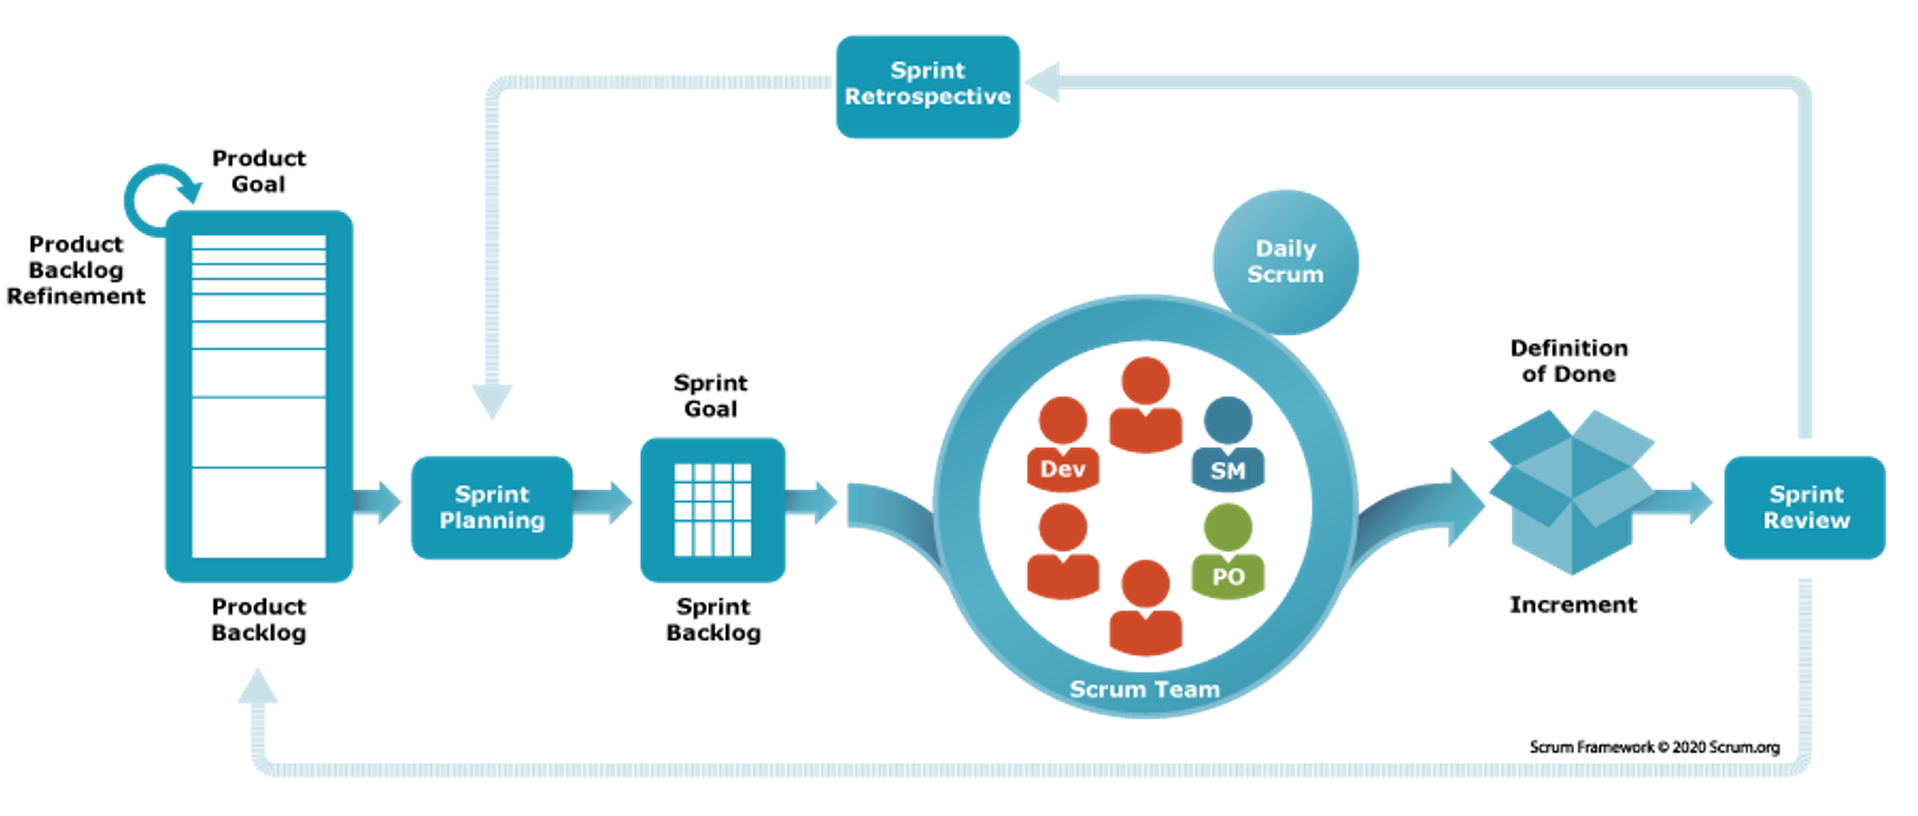
\includegraphics[width=0.9\textwidth]{./img/methodologies/scrum.png}
\caption{Esquema de funcionamiento de Scrum.  Fuente: \href{https://www.scrum.org/learning-series/what-is-scrum/}{Scrum.org}}
\label{fig:scrum}
\end{figure}

\paragraph{Kanban.} Para esta metodología se suele utilizar un tablero visual (\textit{Tablero Kanban}) para representar el flujo de trabajo. Las tareas se representan como tarjetas que se mueven por columnas como \textit{Por hacer}, \textit{En progreso} y \textit{Terminado}. Se establece un límite de trabajo en curso (WIP: Work In Progress, trabajo en progreso) para evitar sobrecargas. Kanban permite detectar cuellos de botella, optimizar procesos y mejorar de forma continua la eficiencia del equipo \cite{kanban}.

\paragraph{Extreme Programming (XP).} XP enfatiza la mejora continua y la satisfacción del cliente \cite{extreme-programming}. Reduce riesgos mediante prácticas técnicas rigurosas:

\begin{enumerate}
    \item Desarrollo iterativo con entregas frecuentes de software funcional.
    \item Pruebas constantes (TDD: Test-Driven Development, desarrollo guiado por tests).
    \item Programación en pareja. Dos desarrolladores trabajan simultáneamente en la misma tarea con el propósito de reducir errores y mejorar el aprendizaje del equipo.
    \item Integración continua.
    \item Código simple y funcional.
    \item Retroalimentación rápida del cliente. El cliente está presente de manera frecuente en el proceso de desarrollo y proporciona su punto de vista para ajustar el desarrollo a sus necesidades
\end{enumerate}

\section{Diseño de la interfaz}

La interfaz ha sido diseñada siguiendo principios de UX/UI centrados en la simplicidad, accesibilidad y claridad visual. Se han creado prototipos en Figma, permitiendo iterar sobre la estructura de navegación, la jerarquía visual y la organización de las secciones: listas, recetas e invitados.

\textbf{Figma} es una herramienta web de diseño de interfaces que permite crear prototipos interactivos, colaborar en tiempo real y compartir diseños entre equipos multidisciplinares. Es ampliamente utilizada en entornos de desarrollo ágil, ya que facilita la comunicación entre diseñadores, desarrolladores y clientes \cite{figma}.

\section{Herramientas de testeo}
\label{sec:test}
Durante el desarrollo se han implementado tests para garantizar la calidad del producto. A continuación se describen los tipos de test implementados y las herramientas utilizadas en cada caso.

\subsection{Test unitarios}

Las pruebas unitarias se centran en comprobar el comportamiento de unidades individuales de código, normalmente funciones, casos de uso o clases, de forma aislada.

\textbf{JUnit4} ha sido la herramienta utiliza para implementar los test unitarios Pinche \cite{android-testing}. Se trata del framework más utilizado en el entorno Kotlin, está ampliamente soportado y cuenta con una buena integración en Android Studio. Junto a JUnit, se ha utilizado \textbf{MockK}, una librería de mocking especialmente diseñada para Kotlin, que permite simular dependencias como repositorios y da soporte para coroutines.

\subsection{Test de interfaz de usuario (UI)}

Los tests de UI tienen como objetivo comprobar cómo se comportan los componentes de la interfaz frente a interacciones del usuario.

Para implementar estos tests en Pinche, se ha utilizado la librería \texttt{androidx.compose.ui:ui-test-junit4}, específica para Jetpack Compose. Permite simular eventos de usuario y verificar la presencia y el estado de los componentes de la vista \cite{android-testing}. Está optimizada para el modelo declarativo de Compose, esto hace que sea la más sencilla al estar ya integrada en el ciclo de vida de la UI de Compose.
